% Created 2014-06-04 Wed 10:40
\documentclass[bigger, presentation]{beamer}
\usepackage[utf8]{inputenc}
\usepackage[T1]{fontenc}
\usepackage{fixltx2e}
\usepackage{graphicx}
\usepackage{longtable}
\usepackage{float}
\usepackage{wrapfig}
\usepackage{soul}
\usepackage{textcomp}
\usepackage{marvosym}
\usepackage{wasysym}
\usepackage{latexsym}
\usepackage{amssymb}
\usepackage{hyperref}
\tolerance=1000
\usepackage{minted}
\usetheme{Frankfurt}   
\usecolortheme[RGB={0,104,139}]{structure}%deepskyblue
\usefonttheme{serif}  % or try serif, structurebold, ...
\setbeamertemplate{navigation symbols}[horizontal]
\setbeamertemplate{caption}[numbered]
\useinnertheme{rounded}
\setbeamercovered{transparent}
\usepackage{pgfpages}
\pgfpagesuselayout{resize to}[physical paper width=8in, physical paper height=6in]
\logo{
\includegraphics[height=0.9cm,width=2cm]{django-logo.png}}
\usepackage{array}
\usepackage{graphicx}
\usepackage{hyperref}
\usepackage[english]{babel}
\usepackage{pxfonts}
\usepackage{listings}
\lstset{numbers=left,numbersep=6pt,numberstyle=\tiny,showstringspaces=false,aboveskip=-50pt,frame=leftline,keywordstyle=\color{black},commentstyle=\color{orange},stringstyle=\color{black},}
\date{today}
\subtitle{Python web framework | Session 3}
\institute{Indian Institute of Technology Bombay}
\providecommand{\alert}[1]{\textbf{#1}}

\title{Django}
\author{Sachin}
\date{\today}
\hypersetup{
  pdfkeywords={org mode, emacs, latex, beamer, pdf},
  pdfsubject={my first presentation made in org mode},
  pdfcreator={Emacs Org-mode version 7.9.3f}}

\begin{document}

\maketitle

\section{pre-sessions}
\label{sec-1}
\begin{frame}
\frametitle{Session 1}
\label{sec-1-1}

   We covered
   
\begin{itemize}
\item Why Python-django
\item Django framework
\item Introduction to \texttt{virtualenv}
\item Install/Configure Django
\item Django views(\texttt{views.py})
\end{itemize}
\end{frame}
\begin{frame}
\frametitle{Session 2}
\label{sec-1-2}

   
   We covered

\begin{itemize}
\item Django admin
\item Models(Databases)
\begin{itemize}
\item \texttt{project/settings.py}
\end{itemize}
\item URLs redirection
\item Templates
\end{itemize}
\end{frame}
\section{url}
\label{sec-2}
\begin{frame}
\frametitle{URL redirection}
\label{sec-2-1}



  \begin{figure}[htb]
  \centering
  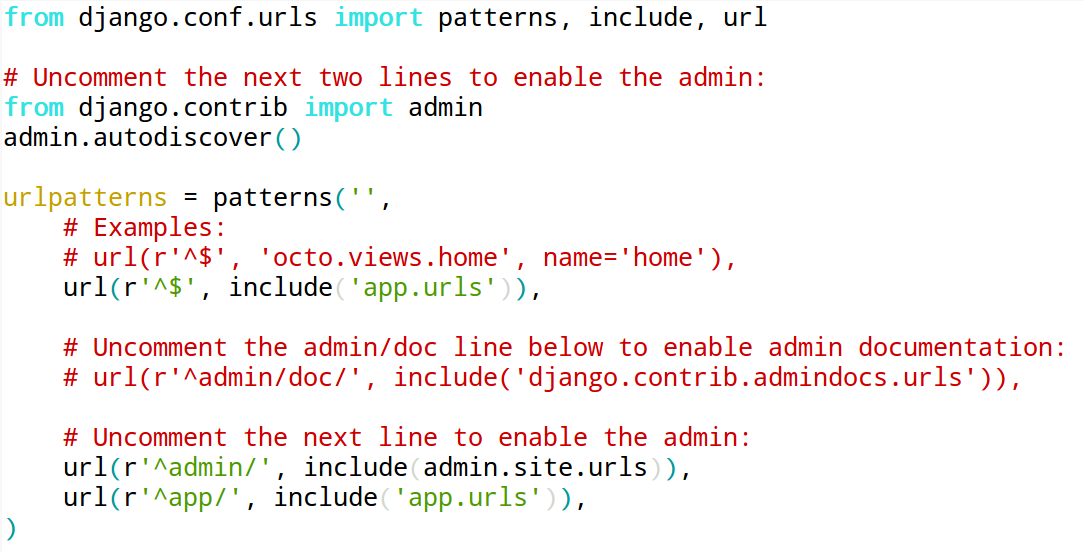
\includegraphics[width=6cm,angle=0]{./project-urls.png}
  \caption{\label{fig:octo/urls.py}\texttt{octo/urls.py}}
  \end{figure}


  \begin{figure}[htb]
  \centering
  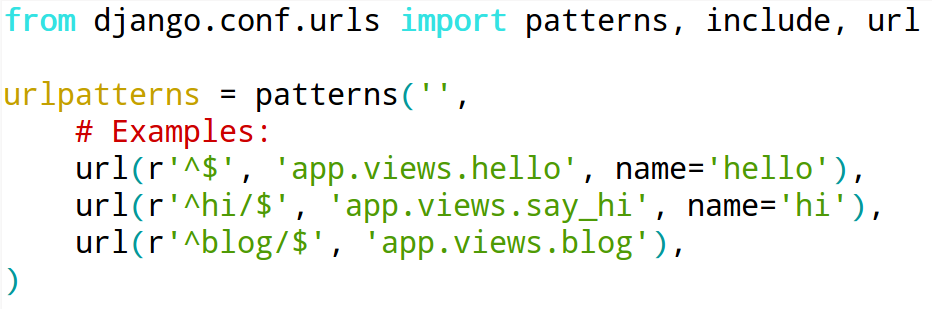
\includegraphics[width=6cm,angle=0]{./apps-urls.png}
  \caption{\label{fig:app/urls.py}\texttt{app/urls.py}}
  \end{figure}
\end{frame}
\section{templates}
\label{sec-3}
\begin{frame}[fragile]
\frametitle{app/views.py}
\label{sec-3-1}



\begin{minted}[]{python}
def blog(request):
    context = RequestContext(request)
    blogs = Blog.objects.all()

    context_dict = {
        'blogs': blogs,
    }

    return render_to_response("app/blog.html",
                              context_dict, context)
\end{minted}
\end{frame}
\begin{frame}[fragile]
\frametitle{List in Python}
\label{sec-3-2}

   

\begin{minted}[]{python}
1:  blogs = ['My first post',
2:          'Started with a BANG!',
3:          'Deep blue Sea',
4:          'Revenge of the fallen']
5:  
6:  print blogs
7:  
8:  for blog in blogs:
9:      print blog
\end{minted}
   
\end{frame}
\begin{frame}[fragile]
\frametitle{Dictionary in Python}
\label{sec-3-3}

   

\begin{minted}[]{python}
1:  context_dict = {
2:      'blogs': blogs,
3:  }
4:  
5:  print context_dict['blogs']
\end{minted}
\end{frame}
\begin{frame}[fragile]
\frametitle{project/templates/app/blog.html}
\label{sec-3-4}



\begin{minted}[]{html}

<h2>{{blog.title}}</h2>
<p>{{blog.body}}</p>

\end{minted}

   
\end{frame}
\section{Forms}
\label{sec-4}
\begin{frame}
\frametitle{Forms in Django}
\label{sec-4-1}

   
\begin{quote}
For lazy nerds
\end{quote}
\end{frame}
\begin{frame}[fragile]
\frametitle{Forms: Decide the url}
\label{sec-4-2}



\begin{minted}[]{sh}
localhost:8000/app/blog/submit
\end{minted}
\end{frame}
\begin{frame}[fragile]
\frametitle{Forms: \texttt{app/urls.py}}
\label{sec-4-3}



\begin{minted}[]{python}
from django.conf.urls import patterns, include, url

urlpatterns = patterns('',
    # ...
    # ...
    url(r'^blog/submit/$', 'app.views.submit_post'),
)
\end{minted}
\end{frame}
\begin{frame}[fragile]
\frametitle{Forms: \texttt{app/views.py}}
\label{sec-4-4}



\begin{minted}[]{python}
def submit_post(request):
    """Create a form to submit post.
    """
    # ..
    return render_to_response()
\end{minted}
\end{frame}
\begin{frame}[fragile]
\frametitle{Forms: \texttt{app/forms.py}}
\label{sec-4-5}



\begin{minted}[]{python}
from django import forms
from models import Blog

# begin forms
class PostForm(forms.ModelForm):
    title = forms.CharField()
    body = forms.TextInput()

    class Meta:
        model = Blog
        fields = ['title', 'body']
\end{minted}
\end{frame}
\begin{frame}[fragile]
\frametitle{Forms: \texttt{app/views.py}}
\label{sec-4-6}



\begin{minted}[]{python}
def submit_post(request):
    """Create a form to submit post.
    """
    # context

    # If user clicked 'Submit' button(POST request)
      # Validate form
        # Save form
        # Show all posts
      # Throw errors(if any)
    # Else show empty form
    return render_to_response()
\end{minted}
\end{frame}
\section{Reference}
\label{sec-5}
\begin{frame}
\frametitle{References}
\label{sec-5-1}

\begin{itemize}
\item \href{https://docs.djangoproject.com/}{https://docs.djangoproject.com/}
\item \href{http://www.tangowithdjango.com/book/}{http://www.tangowithdjango.com/book/}
\end{itemize}
\end{frame}

\end{document}
